\begin{document}
\begin{table*}[t]
\setlength{\abovecaptionskip}{6pt}
\setlength{\belowcaptionskip}{0pt}
    \centering
    \rowcolors{4}{gray!10}{white}
    \adjustbox{max width=\textwidth}{\begin{tabular}{llcc @{\hskip 2mm} c @{\hskip 2mm} c l l | c@{\hskip 2mm} c @{\hskip 2mm}c l l | c @{\hskip 2mm} c @{\hskip 2mm} c  l l}
        \toprule
       & & \multirow{2}{*}[-7pt]{%
  \begin{tabular}[c]{@{}c@{}}%
    {\small \textbf{Densifica-}}\\
    {\small \textbf{tion free}} \\
  \end{tabular}%
}  &\multicolumn{5}{c}{\textbf{Tanks $\&$ Temples}} & \multicolumn{5}{c}{\textbf{Mip-NeRF 360}} &  \multicolumn{5}{c}{\textbf{Deep Blending}}  \\
        \cmidrule(lr){4-18}
                       & &  & \textbf{SSIM} $\uparrow$ & \textbf{PSNR} $\uparrow$ & \textbf{LPIPS} $\downarrow$ & \multicolumn{1}{c}{\begin{tabular}[c]{@{}c@{}}\textbf{Train}\\ \textbf{time}\end{tabular}} &  \multicolumn{1}{c|}{\begin{tabular}[c]{@{}c@{}}\textbf{\#G} \\ ($10^6$)\end{tabular}} &
                          \textbf{SSIM} $\uparrow$& \textbf{PSNR}$\uparrow$ & \textbf{LPIPS}$\downarrow$ & \multicolumn{1}{c}{\begin{tabular}[c]{@{}c@{}}\textbf{Train}\\ \textbf{time}\end{tabular}} &  \multicolumn{1}{c|}{\begin{tabular}[l]{@{}l@{}}\textbf{\#G} \\ ($10^6$)\end{tabular}} &
                          \textbf{SSIM}$\uparrow$ & \textbf{PSNR} $\uparrow$& \textbf{LPIPS} $\downarrow$ & \multicolumn{1}{c}{\begin{tabular}[c]{@{}c@{}}\textbf{Train}\\ \textbf{time}\end{tabular}} &  \multicolumn{1}{l}{\begin{tabular}[c]{@{}c@{}}\textbf{\#G} \\ ($10^6$)\end{tabular}} \\
        \midrule
         \cellcolor{white}& Plenoxels~\cite{fridovich-keil_plenoxels_2022}  &  {\color{ourgreen}\cmark}  & 0.719  & 21.08  & 0.379  & 25 m  & \ \ -  & 0.626  & 23.08  & 0.463  & 26 m  & \ \ -   & 0.795  & 23.06  & 0.510  & 28 m  &  \ \ -  \\
         \cellcolor{white}& INGP-Big~\cite{muller2022instant} &   {\color{ourgreen}\cmark}  & 0.745  & 21.92  & 0.305  & \textbf{7 m } & \ \ - & 0.699  & 25.59  & 0.331  & \textbf{8 m }  & \ \ -   & 0.817  & 24.96  & 0.390  & \textbf{ 8 m}  & \ \ -  \\
          \cellcolor{white} \multirow{-3}{*}{\rotatebox{90}{\textbf{Rays}}}  & Mip-NeRF360~\cite{barron_mip-nerf_2022} &  {\color{ourgreen}\cmark} & 0.759  & 22.22  & 0.257  & 48 h  & \ \ - & 0.792  & 27.69  & 0.237  & 48 h    & \ \ -   & 0.901  & 29.40  & 0.245  & 48 h  & \ \ -  \\

        \midrule
        \cellcolor{white}&3DGS~\cite{kerbl20233d} &  {\color{ourred}\xmark}   & 0.841  & 23.14  & 0.183  & 27 m$^{\ast\ast}$  & 2.0       & 0.815  & 27.21  & 0.214  & 42 m$^{\ast\ast}$    & 3.5  & 0.903  & 29.41  & 0.243  & 36 m$^{\ast\ast}$  & 3.2  \\
        \cellcolor{white}&3DGS~\cite{kerbl20233d}* &  {\color{ourred}\xmark}  & 0.853  & 23.76 & 0.169  & 19 m  & 1.6     & 0.816  & 27.49  & 0.215  & 26 m    & \underline{2.8}  & \textbf{0.908}  & 29.77  & 0.242  &  27 m &  2.6 \\
        \cellcolor{white}& AbsGS-0004~\cite{ye2024absgs} &  {\color{ourred}\xmark} & 0.852  & 23.59  & 0.162  & 14 m  & \textbf{1.4}   & 0.818  & 27.41  & 0.198 & \underline{20 m}    & 3.1    & 0.901  & 29.61  & \underline{0.236}  & 20 m  & \underline{1.9}  \\
        \cellcolor{white} & Rain-GS~\cite{jung2024relaxing}$^{\dagger}$ &  {\color{ourred}\xmark} &  0.823 & 23.13 & 0.207  & 15 m$^{\star \star}$  & \ \ -  &  0.807  & 27.23  & 0.229  &  32 m$^{\star \star}$    & \ \ -   & 0.900  &  29.42 & 0.255  & 28 m$^{\star \star}$  & \ \ - \\
        \cellcolor{white} & Mip-Splatting~\cite{yu2024mip} &  {\color{ourred}\xmark} & 0.859  & 23.81  & \underline{0.156}  & 16 m  & 2.4  & 0.838  & 27.97  & 0.179  &  26 m   & 4.0  &  0.903 & 29.35 & 0.239  & 29 m  &  3.6 \\
        \cellcolor{white} & 3DGS-MCMC~\cite{kheradmand20243d} &  {\color{ourred}\xmark} &  \underline{0.863} & \underline{24.22}  & 0.158  & \underline{13 m}  & \underline{1.9}  &  \textbf{0.842} &  \textbf{28.15} &   \underline{0.176}   &  \underline{20 m} & 3.2   & 0.902  & 29.56  & 0.244  & \underline{19 m} & 2.9 \\
        \cellcolor{white}& ScaffoldGS~\cite{lu2024scaffold} &  {\color{ourred}\xmark}  & 0.854 & 24.08  & 0.165  & 23 m  & 6.0$^\ddagger$   & 0.812  & 27.60  & 0.222  & 22 m    & 6.0$^\ddagger$  & \underline{0.907}  &  \textbf{30.25} & 0.245  & 28 m  & 4.0$^\ddagger$  \\

        \cmidrule(lr){2-18}
        \cellcolor{white} \multirow{-7}{*}{\rotatebox{90}{\textbf{ \quad Gaussians}}}&\cellcolor{white}  \textbf{EDGS + 3DGS} &  \cellcolor{white} {\color{ourgreen}\cmark} & \cellcolor{white} \textbf{0.868} & \cellcolor{white} \textbf{24.28} &  \cellcolor{white} \textbf{0.132} & \cellcolor{white} 23 m & \cellcolor{white} \textbf{1.4} & \cellcolor{white} \underline{0.839} & \cellcolor{white} \underline{28.02} & \cellcolor{white} \textbf{0.141} & \cellcolor{white} 27 m & \cellcolor{white} \textbf{1.9}   &
                         \cellcolor{white} 0.904  & \cellcolor{white} \underline{29.81} & \cellcolor{white} \textbf{0.223} & \cellcolor{white} 30 m & \cellcolor{white} \textbf{1.6} \\
        \bottomrule
       \multicolumn{18}{c}{\cellcolor{white} {\small $^\dagger$ results were taken directly from the paper, $^\ddagger$ for ScaffoldGS denotes the number of splats produced by anchors, $^{\ast \ast}$ results reported for an NVIDIA A6000, $^{\star \star}$ results or an NVIDIA RTX 3090.}} \\
    \end{tabular}}
   \caption{Performance comparison on Mip-NeRF 3.}
    \label{tab:merged_comparison}
\end{table*}
\begin{table}[t]
    \centering
    \adjustbox{max width=0.47\textwidth}{\begin{tabular}{c c c @{\hskip 2mm} c @{\hskip 2mm} c @{\hskip 2mm} c @{\hskip 2mm}c l }
    \toprule
     \multicolumn{2}{c}{\cellcolor{white}\textbf{Mip-NeRF 360}} & \multicolumn{1}{c}{\begin{tabular}[c]{@{}c@{}}\textbf{Densif.}\\ \textbf{free}\end{tabular}}& \textbf{SSIM} $\uparrow$ & \textbf{PSNR} $\uparrow$ & \textbf{LPIPS} $\downarrow$ & \multicolumn{1}{c}{\begin{tabular}[c]{@{}c@{}}\textbf{Train}\\ \textbf{time}\end{tabular}} &  \multicolumn{1}{c}{\begin{tabular}[c]{@{}c@{}}\textbf{\#G} \\ ($10^6$)\end{tabular}}  \\
    \midrule
    & gsplat~\cite{ye2024gsplatopensourcelibraryGaussian} &  {\color{ourred}\xmark}   & 0.818  & 27.51  & 0.215  & 18 m    & 3.1  \\
   \cellcolor{white} & 3DGS+3DGS-LM~\cite{hollein20243dgs}$^\dagger$ &  {\color{ourred}\xmark} &   0.813  & 27.39  & 0.221  & 16 m    & 2.8$^{\star}$ \\
    & EAGLES~\cite{girish2023eagles} &  {\color{ourred}\xmark}  & 0.809 &  27.20 & 0.232  &  16 m   &  \underline{1.3}   \\
    \cellcolor{white} & Taming 3DGS~\cite{mallick2024taming} &  {\color{ourred}\xmark}  & 0.820  & \textbf{27.71}  & 0.207  &  14 m   & 3.2   \\
    & MiniSplatting~\cite{Fang2024MiniSplattingRS} &  {\color{ourred}\xmark}  & 0.820  &  27.25 & 0.217  &  \underline{12 m}   & \textbf{0.5}  \\
    & \textbf{EDGS + 3DGS 10K} & {\color{ourgreen}\cmark} & \textbf{0.834} & \underline{27.54} & \textbf{0.154} & \underline{12 m} & 2.1 \\
   \multirow{-8}{*}{
\cellcolor{white}
\makebox[0pt][c]{%
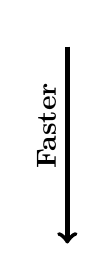
\begin{tikzpicture}[baseline=(A.base)]
  \node (A) {};
  \draw[->, ultra thick] (A.south) -- ++(0,-2.5)
    node[midway, above=7pt, font=\bfseries, rotate=90,]{Faster};
\end{tikzpicture}
}}  & \textbf{EDGS + 3DGS 5K}  & {\color{ourgreen}\cmark} & \underline{0.825} & 26.88 & \underline{0.166} & \textbf{8 m} & 2.6
                      \\
        \bottomrule
         \multicolumn{8}{c}{\cellcolor{white} {\small
         $^\dagger$~From original paper. $^\star$~Assumed same as 3DGS~\cite{kerbl20233d} due to identical densification.}}
    \end{tabular}}
    \caption{Quantitative evaluation under early-stopping settings on Mip-NeRF 360~\cite{barron_mip-nerf_2022}. When trained for a comparable duration (\textit{EDGS 10K}), our method outperforms other efficient approaches. Even with reduced training time (\textit{EDGS 5K}), it outperforms all competing methods on two of the three standard metrics.}
    \label{tab:efficciency_comparison}
\end{table}
\begin{table}[ht]
    \centering
    \adjustbox{max width=0.47\textwidth}{\begin{tabular}{l@{\hskip 2mm} c @{\hskip 2mm} l @{\hskip 2mm} l@{\hskip 2mm} l @{\hskip 2mm} l  l}
        \toprule
                     \textbf{Mip-NeRF 360} & \multicolumn{1}{c}{\begin{tabular}[c]{@{}c@{}}\textbf{EDGS}\\ \textbf{Init}\end{tabular}} & \textbf{SSIM} $\uparrow$ & \textbf{PSNR} $\uparrow$ & \multicolumn{1}{c}{\textbf{LPIPS} $\downarrow$} & \multicolumn{1}{c}{\begin{tabular}[c]{@{}c@{}}\textbf{Train}\\ \textbf{time}\end{tabular}} &  \multicolumn{1}{c}{\begin{tabular}[c]{@{}c@{}}\textbf{\#G} \\ ($10^6$)\end{tabular}} \\
        \midrule
         &  {\color{ourred}\xmark}  & 0.818  & 27.41  & 0.198 & 20 m    & 3.1 \\
         \multirow{-2}[0]{*}{AbsGS-0004~\cite{ye2024absgs}} &  {\color{ourgreen}\cmark}  & 0.822\textsubscript{\color{ourgreen}$\blacktriangle1\%$} & 27.53\textsubscript{\color{ourgreen}$\blacktriangle 0.12$} & 0.187\textsubscript{\color{ourgreen}$\blacktriangledown$6\%} & 19 m & 3.0  \\
        \rowcolor{gray!10}  &  {\color{ourred}\xmark} &  0.842 &  28.15 &   0.176   &  20 m & 3.2 \\
        \rowcolor{gray!10} \multirow{-2}[0]{*}{3DGS-MCMC~\cite{kheradmand20243d}} &  {\color{ourgreen}\cmark} & 0.847\textsubscript{\color{ourgreen}$\blacktriangle 1\%$} & 28.29\textsubscript{\color{ourgreen}$\blacktriangle 0.14$} & 0.159\textsubscript{\color{ourgreen}$\blacktriangledown$10\%} & 20 m & 3.2  \\
        &  {\color{ourred}\xmark} & 0.820  & 27.71  & 0.207  &  14 m   & 3.2 \\
       \multirow{-2}[0]{*}{Taming 3DGS~\cite{mallick2024taming}} &  {\color{ourgreen}\cmark}  & 0.842\textsubscript{\color{ourgreen}$\blacktriangle 3\%$} & 28.07\textsubscript{\color{ourgreen}$\blacktriangle 0.36$} & 0.179\textsubscript{\color{ourgreen}$\blacktriangledown$14\%} & 11 m & 3.2 \\
        \bottomrule
    \end{tabular}}
    \caption{EDGS as initialization for different densification methods. Incorporating our approach, without fine-tuning hyperparameters and across various settings, consistently improves all other methods without increasing final Gaussian count or increasing training time. For \textit{EDGS Init}, the reported time includes the initialization phase. }
    \label{tab:ours_plus_adc}
\end{table}
\end{document}
